\documentclass[12pt,a4paper]{article}
\usepackage[utf8]{vietnam}
\usepackage{amsmath,amssymb}
\usepackage{tabularx}
\usepackage{tikz}
\usetikzlibrary{calc,angles,quotes,arrows.meta,patterns}
\usepackage{xcolor}
\usepackage{enumitem}
\usepackage{fancyhdr}
\usepackage[top=1.2cm, bottom=1.2cm, left=1.5cm, right=1.5cm]{geometry}
\usepackage[loigiai]{ex_test}
\SAOPTN{widthSA=2.6,heightSA=0.62}

\setlength{\headheight}{15pt}
\setlength{\parskip}{0pt}

\pagestyle{fancy}
\fancyhf{}
\rhead{\textit{Môn Toán 6 -- Hướng dẫn giải Đề số 3}}
\lhead{\textit{Bộ đề ôn tập Giữa học kì I}}
\cfoot{\thepage}

\begin{document}

\begin{center}
  \textbf{\Large HƯỚNG DẪN GIẢI CHI TIẾT VÀ BẢNG ĐÁP ÁN}\\
  \textbf{\large ĐỀ ÔN TẬP GIỮA HỌC KỲ I -- ĐỀ SỐ 3}\\
  \textit{Môn: Toán 6 -- Năm học 2026 -- 2027}
\end{center}
\vspace{2mm}

% --- BẢNG ĐÁP ÁN TRẮC NGHIỆM TỔNG HỢP ---
\noindent\textbf{\large A. BẢNG ĐÁP ÁN TRẮC NGHIỆM TỔNG HỢP}
\vspace{1.5mm}

\noindent\textbf{1. Phần I (Mỗi câu trả lời đúng được 0,25 điểm):}
\begin{center}
\begin{tabular}{|c|c|c|c|c|c|c|c|c|c|c|c|c|}
\hline
\textbf{Câu} & \textbf{1} & \textbf{2} & \textbf{3} & \textbf{4} & \textbf{5} & \textbf{6} & \textbf{7} & \textbf{8} & \textbf{9} & \textbf{10} & \textbf{11} & \textbf{12} \\
\hline
\textbf{Đ/A} & \textbf{D} & \textbf{C} & \textbf{A} & \textbf{C} & \textbf{B} & \textbf{B} & \textbf{A} & \textbf{C} & \textbf{C} & \textbf{A} & \textbf{D} & \textbf{A} \\
\hline
\end{tabular}
\end{center}
\vspace{1mm}

\noindent\textbf{2. Phần II (Đúng/Sai):}
\begin{center}
\begin{tabular}{|c|c|c|c|c||c|c|c|c|c|}
\hline
\textbf{Câu 1} & \textbf{a)} & \textbf{b)} & \textbf{c)} & \textbf{d)} & \textbf{Câu 2} & \textbf{a)} & \textbf{b)} & \textbf{c)} & \textbf{d)} \\
\hline
\textbf{Đ/S} & \textbf{Đ} & \textbf{S} & \textbf{S} & \textbf{Đ} & \textbf{Đ/S} & \textbf{Đ} & \textbf{S} & \textbf{S} & \textbf{Đ} \\
\hline
\end{tabular}
\end{center}
\vspace{1mm}

\noindent\textbf{3. Phần III (Mỗi câu trả lời đúng được 1,0 điểm):}
\begin{center}
\begin{tabular}{|c|c|c|}
\hline
\textbf{Câu} & \textbf{Câu 1} & \textbf{Câu 2} \\
\hline
\textbf{Đáp án} & \textbf{4} & \textbf{8} \\
\hline
\end{tabular}
\end{center}
\vspace{3mm}

% --- LỜI GIẢI CHI TIẾT ---
\noindent\textbf{\large B. HƯỚNG DẪN GIẢI CHI TIẾT TỪNG CÂU}
\vspace{2mm}

\noindent\textbf{\large PHẦN I. CÂU TRẮC NGHIỆM NHIỀU PHƯƠNG ÁN LỰA CHỌN}
\vspace{1mm}
\begin{ex}
Cho tập hợp $A = \{1; 2; a; b\}$. Khẳng định nào dưới đây là sai?
\choice
{$1 \in A$}
{$a \in A$}
{$5 \notin A$}
{\True $b \notin A$}
\loigiai{
Vì $b$ là một phần tử thuộc tập hợp $A$ nên khẳng định đúng là $b \in A$. Do đó khẳng định $b \notin A$ là sai.
}
\end{ex}

\begin{ex}
Tập hợp nào dưới đây là tập hợp số tự nhiên?
\choice
{$\mathbb{N} = \{1; 2; 3; \dots\}$}
{$\mathbb{N} = \{0; 1; 2; 3; \dots; 100\}$}
{\True $\mathbb{N} = \{0; 1; 2; 3; \dots\}$}
{$\mathbb{N} = \{0; 2; 4; 6; \dots\}$}
\loigiai{
Tập hợp các số tự nhiên kí hiệu là $\mathbb{N} = \{0; 1; 2; 3; \dots\}$.
}
\end{ex}

\begin{ex}
Số nào sau đây là bội của $17$?
\choice
{\True $51$}
{$54$}
{$56$}
{$63$}
\loigiai{
Ta có $51 = 17 \times 3 \implies 51 \ \vdots \ 17$ nên $51$ là bội của $17$.
}
\end{ex}

\begin{ex}
Một nhà kho có $240$ bao gạo, chia đều vào $8$ dãy kệ. Sau đó, người ta lấy ra $15$ bao ở mỗi dãy kệ để chuyển đi nơi khác. Hỏi nhà kho còn lại bao nhiêu bao gạo?
\choice
{$105$ bao}
{$115$ bao}
{\True $120$ bao}
{$135$ bao}
\loigiai{
Mỗi dãy kệ lúc đầu có: $240 : 8 = 30$ (bao). Sau khi lấy ra 15 bao, mỗi dãy còn: $30 - 15 = 15$ (bao). Số bao gạo còn lại trong kho là: $15 \times 8 = 120$ (bao).
}
\end{ex}

\begin{ex}
Công thức tính chu vi của hình vuông có độ dài cạnh $a$ là:
\choice
{$C = a$}
{\True $C = 4a$}
{$C = 3a$}
{$C = 5a$}
\loigiai{
Chu vi của hình vuông cạnh $a$ là tổng độ dài bốn cạnh bằng nhau: $C = 4a$.
}
\end{ex}

\begin{ex}
Trong các hình dưới đây, hình nào là hình thoi?\begin{center}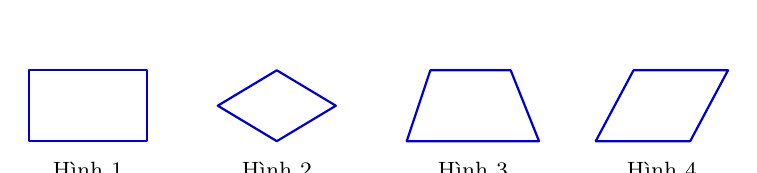
\begin{tikzpicture}[scale=0.6, line cap=round, line join=round]\begin{scope}[xshift=0cm]\draw[thick, blue!80!black] (0,0) rectangle (2.5,1.5);\node[below=4pt, font=\footnotesize] at (1.25,0) {Hình 1};\end{scope}\begin{scope}[xshift=4cm]\draw[thick, blue!80!black] (1.25,1.5) -- (2.5,0.75) -- (1.25,0) -- (0,0.75) -- cycle;\node[below=4pt, font=\footnotesize] at (1.25,0) {Hình 2};\end{scope}\begin{scope}[xshift=8cm]\draw[thick, blue!80!black] (0.5,1.5) -- (2.2,1.5) -- (2.8,0) -- (0,0) -- cycle;\node[below=4pt, font=\footnotesize] at (1.4,0) {Hình 3};\end{scope}\begin{scope}[xshift=12cm]\draw[thick, blue!80!black] (0.8,1.5) -- (2.8,1.5) -- (2,0) -- (0,0) -- cycle;\node[below=4pt, font=\footnotesize] at (1.4,0) {Hình 4};\end{scope}\end{tikzpicture}\end{center}
\choice
{Hình 1}
{\True Hình 2}
{Hình 3}
{Hình 4}
\loigiai{
Hình 1 là hình chữ nhật, Hình 2 là hình thoi (có 4 cạnh bằng nhau), Hình 3 là hình thang, Hình 4 là hình bình hành.
}
\end{ex}

\begin{ex}
Đọc lũy thừa $6^3$ và nêu cơ số, số mũ của nó:
\choice
{\True Sáu mũ ba; cơ số là $6$, số mũ là $3$}
{Sáu mũ ba; cơ số là $3$, số mũ là $6$}
{Ba mũ sáu; cơ số là $3$, số mũ là $6$}
{Ba mũ sáu; cơ số là $6$, số mũ là $3$}
\loigiai{
Lũy thừa $6^3$ đọc là "sáu mũ ba" (hoặc "sáu lũy thừa ba"); cơ số là $6$ và số mũ là $3$.
}
\end{ex}

\begin{ex}
Khi viết gọn tích $3 \cdot 2 \cdot 6^2 \cdot 6$ dưới dạng một lũy thừa, kết quả đúng là:
\choice
{$3^3 \cdot 2^2$}
{$6^3$}
{\True $6^4$}
{$2^3 \cdot 3^2$}
\loigiai{
Ta có: $3 \cdot 2 \cdot 6^2 \cdot 6 = 6 \cdot 6^2 \cdot 6 = 6^{1 + 2 + 1} = 6^4$.
}
\end{ex}

\begin{ex}
Khẳng định nào sau đây là đặc trưng về cạnh của hình vuông?
\choice
{Hai cạnh đối bằng nhau}
{Hai đường chéo bằng nhau}
{\True Bốn cạnh bằng nhau}
{Hai đường chéo vuông góc}
\loigiai{
Hình vuông có bốn cạnh bằng nhau và bốn góc bằng nhau (bằng $90^\circ$).
}
\end{ex}

\begin{ex}
Cho hình thang có độ dài hai đáy lần lượt là $6\text{ cm}$ và $10\text{ cm}$, chiều cao là $5\text{ cm}$. Diện tích của hình thang đó là:
\choice
{\True $40\text{ cm}^2$}
{$50\text{ cm}^2$}
{$60\text{ cm}^2$}
{$70\text{ cm}^2$}
\loigiai{
Diện tích hình thang là: $S = \dfrac{(a + b) \cdot h}{2} = \dfrac{(6 + 10) \cdot 5}{2} = \dfrac{16 \cdot 5}{2} = 40\text{ cm}^2$.
}
\end{ex}

\begin{ex}
Cho tam giác đều $MNP$ có cạnh $MP = 6\text{ cm}$. Độ dài các cạnh $MN$ và $NP$ lần lượt là:
\choice
{$2\text{ cm}; 4\text{ cm}$}
{$3\text{ cm}; 3\text{ cm}$}
{$1\text{ cm}; 5\text{ cm}$}
{\True $6\text{ cm}; 6\text{ cm}$}
\loigiai{
Tam giác đều $MNP$ có 3 cạnh bằng nhau nên $MN = NP = MP = 6\text{ cm}$.
}
\end{ex}

\begin{ex}
Một hình thoi có độ dài hai đường chéo lần lượt là $2\text{ cm}$ và $4\text{ cm}$. Diện tích của hình thoi đó là:
\choice
{\True $4\text{ cm}^2$}
{$6\text{ cm}^2$}
{$8\text{ cm}^2$}
{$2\text{ cm}^2$}
\loigiai{
Diện tích hình thoi là: $S = \dfrac{m \cdot n}{2} = \dfrac{2 \cdot 4}{2} = 4\text{ cm}^2$.
}
\end{ex}


\setcounter{ex}{0}
\noindent\textbf{\large PHẦN II. CÂU TRẮC NGHIỆM ĐÚNG SAI}
\vspace{1mm}
\begin{ex}
Cho hình vuông $MNPQ$ có cạnh bằng $4\text{ cm}$. Các khẳng định sau đây đúng hay sai?
\choiceTF
{\True $MN = NP = PQ = QM = 4\text{ cm}$}
{$MN$ và $NQ$ song song với nhau}
{Mỗi góc ở các đỉnh của hình vuông bằng nhau và bằng $60^\circ$}
{\True Dùng thước và ê-ke vẽ được hình vuông $MNPQ$ có cạnh bằng $4\text{ cm}$}
\loigiai{
\begin{itemize}[leftmargin=0.6cm, itemsep=1pt]
\item \textbf{a)} \textbf{Đúng}. Hình vuông có bốn cạnh bằng nhau và bằng 4 cm. Khẳng định đúng.
\item \textbf{b)} \textbf{Sai}. $MN$ và $NQ$ cắt nhau tại đỉnh $N$, không song song. Khẳng định sai.
\item \textbf{c)} \textbf{Sai}. Mỗi góc ở các đỉnh của hình vuông bằng $90^\circ$. Khẳng định sai.
\item \textbf{d)} \textbf{Đúng}. Dùng thước và ê-ke hoàn toàn xác định được các góc vuông và độ dài 4 cm. Khẳng định đúng.
\end{itemize}
}
\end{ex}

\begin{ex}
Cho các số: $355, 360, 257, 1617, 152$. Các khẳng định sau đây đúng hay sai?
\choiceTF
{\True Số $360$ chia hết cho $9$}
{Số $1617$ chia hết cho $9$}
{Trong các số đã cho, có đúng hai số chia hết cho $9$}
{\True Số $257$ và số $152$ đều không chia hết cho $9$}
\loigiai{
\begin{itemize}[leftmargin=0.6cm, itemsep=1pt]
\item \textbf{a)} \textbf{Đúng}. Tổng các chữ số của 360 là $3 + 6 + 0 = 9 \ \vdots \ 9$. Khẳng định đúng.
\item \textbf{b)} \textbf{Sai}. Tổng các chữ số là $1 + 6 + 1 + 7 = 15$ không chia hết cho 9. Khẳng định sai.
\item \textbf{c)} \textbf{Sai}. Chỉ có duy nhất số 360 chia hết cho 9. Khẳng định sai.
\item \textbf{d)} \textbf{Đúng}. Tổng các chữ số: $2+5+7=14$ và $1+5+2=8$ đều không chia hết cho 9. Khẳng định đúng.
\end{itemize}
}
\end{ex}


\setcounter{ex}{0}
\noindent\textbf{\large PHẦN III. CÂU HỎI TRẢ LỜI NGẮN}
\vspace{1mm}
\begin{ex}
Số lượng các số nguyên tố nhỏ hơn $10$ là bao nhiêu? \shortans{$4$}
\loigiai{
Các số nguyên tố nhỏ hơn 10 là $\{2; 3; 5; 7\}$. Vậy có $4$ số.
}
\end{ex}

\begin{ex}
Có bao nhiêu số tự nhiên $n$ thỏa mãn $1 < n \le 9$? \shortans{$8$}
\loigiai{
Các số tự nhiên thỏa mãn là $\{2; 3; 4; 5; 6; 7; 8; 9\}$. Số lượng phần tử là $9 - 2 + 1 = 8$ (số).
}
\end{ex}


\setcounter{ex}{0}
\noindent\textbf{\large PHẦN IV. TỰ LUẬN (3,0 ĐIỂM - CÓ BAREM ĐIỂM CHI TIẾT)}
\vspace{1mm}
\begin{ex} (1.0 điểm)
Thực hiện phép tính:
\begin{enumerate}[label=\textbf{\alph*)}, leftmargin=0.8cm, itemsep=2pt]
\item $475 + 170 + 325 + 330$
\item $89 \cdot 54 + 45 \cdot 89 + 89$
\item $120 : \left\{ 54 - \left[ 50 : 2 - (3^2 - 2 \cdot 4) \right] \right\}$
\end{enumerate}
\loigiai{
\begin{itemize}[leftmargin=0.5cm, itemsep=3pt]
\item \textbf{a)} $475 + 170 + 325 + 330 = (475 + 325) + (170 + 330) = 800 + 500 = 1300$. \hfill \textbf{[0.25đ]}
\item \textbf{b)} $89 \cdot 54 + 45 \cdot 89 + 89 = 89 \cdot (54 + 45 + 1) = 89 \cdot 100 = 8900$. \hfill \textbf{[0.25đ]}
\item \textbf{c)} $120 : \left\{ 54 - \left[ 25 - (9 - 8) \right] \right\} = 120 : \left\{ 54 - \left[ 25 - 1 \right] \right\} = 120 : \left\{ 54 - 24 \right\} = 120 : 30 = 4$. \hfill \textbf{[0.5đ]}
\end{itemize}
}
\end{ex}
\vspace{1.5mm}

\begin{ex} (0.75 điểm)
Tìm số tự nhiên $x$, biết:
\begin{enumerate}[label=\textbf{\alph*)}, leftmargin=0.8cm, itemsep=2pt]
\item $x - 15 = 2025$
\item $39 + (x - 47) = 160$
\end{enumerate}
\loigiai{
\begin{itemize}[leftmargin=0.5cm, itemsep=3pt]
\item \textbf{a)} $x = 2025 + 15 \implies x = 2040$. \hfill \textbf{[0.25đ]}
\item \textbf{b)} $x - 47 = 160 - 39$\
$x - 47 = 121$\
$x = 121 + 47 = 168$. \hfill \textbf{[0.5đ]}
\end{itemize}
}
\end{ex}
\vspace{1.5mm}

\begin{ex} (0.75 điểm)
Mảnh vườn nhà ông An có dạng như hình vẽ dưới đây:\
\begin{center}
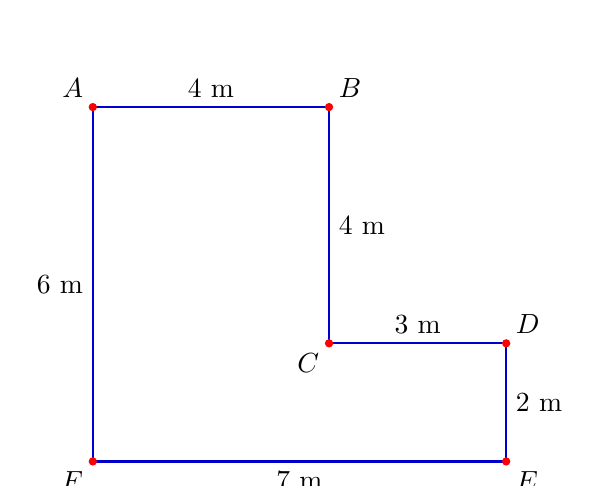
\begin{tikzpicture}[scale=0.75, line cap=round, line join=round]
  \coordinate (F) at (0,0); \coordinate (E) at (7,0); \coordinate (D) at (7,2);
  \coordinate (C) at (4,2); \coordinate (B) at (4,6); \coordinate (A) at (0,6);
  \draw[thick, blue!80!black] (F) -- (E) -- (D) -- (C) -- (B) -- (A) -- cycle;
  \foreach \p in {A,B,C,D,E,F} \fill[red] (\p) circle (2pt);
  \node[above left] at (A) {$A$};
  \node[above right] at (B) {$B$};
  \node[below left] at (C) {$C$};
  \node[above right] at (D) {$D$};
  \node[below right] at (E) {$E$};
  \node[below left] at (F) {$F$};
  \node[above] at (2,6) {$4\text{ m}$};
  \node[right] at (4,4) {$4\text{ m}$};
  \node[above] at (5.5,2) {$3\text{ m}$};
  \node[right] at (7,1) {$2\text{ m}$};
  \node[below] at (3.5,0) {$7\text{ m}$};
  \node[left] at (0,3) {$6\text{ m}$};
\end{tikzpicture}
\end{center}
\begin{enumerate}[label=\textbf{\alph*)}, leftmargin=0.8cm, itemsep=2pt]
\item Ông An rào xung quanh mảnh vườn bằng dây thép gai. Hỏi ông An mua hết bao nhiêu tiền dây thép gai, biết mỗi mét dây thép gai có giá $50\,000$ đồng?
\item Tính diện tích mảnh vườn của ông An.
\end{enumerate}
\loigiai{
\begin{itemize}[leftmargin=0.5cm, itemsep=3pt]
\item \textbf{a)} Chu vi mảnh vườn hình chữ L là:\
$C = AB + BC + CD + DE + EF + FA = 4 + 4 + 3 + 2 + 7 + 6 = 26\text{ (m)}$.\
Số tiền mua dây thép gai để rào hết xung quanh mảnh vườn là:\
$26 \times 50\,000 = 1\,300\,000\text{ (đồng)}$. \hfill \textbf{[0.5đ]}
\item \textbf{b)} Chia mảnh vườn thành hai hình chữ nhật: hình chữ nhật thứ nhất kích thước $4\text{ m} \times 6\text{ m}$ và hình chữ nhật thứ hai kích thước $3\text{ m} \times 2\text{ m}$.\
Diện tích mảnh vườn của ông An là:\
$S = 4 \times 6 + 3 \times 2 = 24 + 6 = 30\text{ (m}^2\text{)}$. \hfill \textbf{[0.25đ]}
\end{itemize}
}
\end{ex}
\vspace{1.5mm}

\begin{ex} (0.5 điểm)
Cho tổng $B = 5 + 5^2 + 5^3 + \dots + 5^8$. Chứng minh rằng $B$ chia hết cho $30$.
\begin{enumerate}[label=\textbf{\alph*)}, leftmargin=0.8cm, itemsep=2pt]
\item Chứng minh $B \ \vdots \ 30$.
\end{enumerate}
\loigiai{
\begin{itemize}[leftmargin=0.5cm, itemsep=3pt]
\item \textbf{a)} Ta nhóm hai số hạng liên tiếp với nhau:\
$B = (5 + 5^2) + (5^3 + 5^4) + (5^5 + 5^6) + (5^7 + 5^8)$\
$B = 5 \cdot (1 + 5) + 5^3 \cdot (1 + 5) + 5^5 \cdot (1 + 5) + 5^7 \cdot (1 + 5)$\
$B = 5 \cdot 6 + 5^3 \cdot 6 + 5^5 \cdot 6 + 5^7 \cdot 6$\
$B = 30 + 30 \cdot 5^2 + 30 \cdot 5^4 + 30 \cdot 5^6$\
$B = 30 \cdot (1 + 5^2 + 5^4 + 5^6)$.\
Vì $30 \ \vdots \ 30$ nên $B \ \vdots \ 30$ (đpcm). \hfill \textbf{[0.5đ]}
\end{itemize}
}
\end{ex}
\vspace{1.5mm}


\begin{center}
\rule{4cm}{0.4pt}\\
\textit{--- HẾT ---}
\end{center}
\end{document}
